\chapter{Transposable element co-option}
\label{chap:mer130}

\section{Introduction}

Transcriptional enhancers control when, where, and how much of each gene
is produced in different cell types at different
times~\citep{Levo:2014hl}. Together, groups of enhancers orchestrate the
expression of many genes to form complex pathways, but a fundamental
question is what produced this coordinated regulatory logic. Instances
of recognizable transposable element (TE) families make up more than
half the human genome~\citep{Wheeler:2012im}, providing a large substrate of
homologous sequences on which evolution can act.

In 1969, Roy Britten and Eric Davidson proposed a mechanism by which the
evolution of novel structures or functions could be greatly accelerated
through the co-option of TEs into gene regulatory roles, activating
novel groups of genes that were not co-expressed before in a new
temporally and spatially-specific manner~\citep{Britten:1971tl}. By
scattering copies of the same DNA stretches across the genome near all
manner of genes, TEs could greatly increase the probability that groups
of enhancers would emerge to bring together a new group of genes, to be
expressed together and accelerate the formation of complex new pathways
and functions. Consistent with the idea of TEs seeding regulatory
sequences, TEs have contributed significantly to conserved non-coding
elements, via their co-option into gene regulatory
roles~\citep{Lowe:2007je}. In addition, TE families have been co-opted in
different contexts such as stem cells~\citep{Kunarso:2010kt} and the
placenta~\citep{Chuong:2013hj}.

p300 is a transcriptional co-activator recruited by active enhancers. It
is an appealing epigenomic mark of active enhancers, with typical
\emph{in vivo} validation rates of 80\%~\citep{May:2012iy}. In a recent
paper~\citep{Wenger:2013jd}, we measured the p300 landscape of the E14.5
dorsal cerebral wall (DCW), which encompasses and gives rise to the
neocortex, by harvesting tissue from mouse embryos, isolating chromatin,
and performing chromatin immunoprecipitation followed by high-throughput
sequencing (ChIP-seq). In that study, we used multiple techniques to
validate the quality of our p300 measurements, including confirming key
enhancers known from the literature and enrichment analysis showing that
from thousands of measured tissue-timepoint combinations, our set is
most correlated with genes expressed in Theiler stage 22 telencephalon
(essentially E14.5 DCW). Using transgenics, we confirmed that 8 of 10
(80\%) p300 measurements function as active neocortical enhancers, and
established a primary cortical neuron transfection system where 5/8
positive transgenics showed transfection activity, and 2/2 negative
transgenics did not~\citep{Wenger:2013jd}.

Here we show that the MER130 repeat family is strongly enriched among
the E14.5 enhancers in the developing neocortex, an enrichment that is
specific to mouse brain tissues. MER130 is a nonautonomous interspersed
repeat family that previously has been shown to be conserved in mammals
and chicken~\citep{Jurka:2005bl}. In pursuit of the Britten \& Davidson
hypothesis, we show that the activity of MER130 family members is the
result of a preserved core of regulatory logic that consists of multiple
transcription factor binding sites. Individual MER130 instances function
as enhancers, although we show that the endogenous chromatin state is
essential to interpreting these results. Furthermore, MER130 instances
that function as enhancers lie next to important cortical genes, yet are
conserved to species that far predate the emergence of the neocortex.

\section{Results}

\begin{figure}[htbp]
\centering
\begin{tabular}{l}
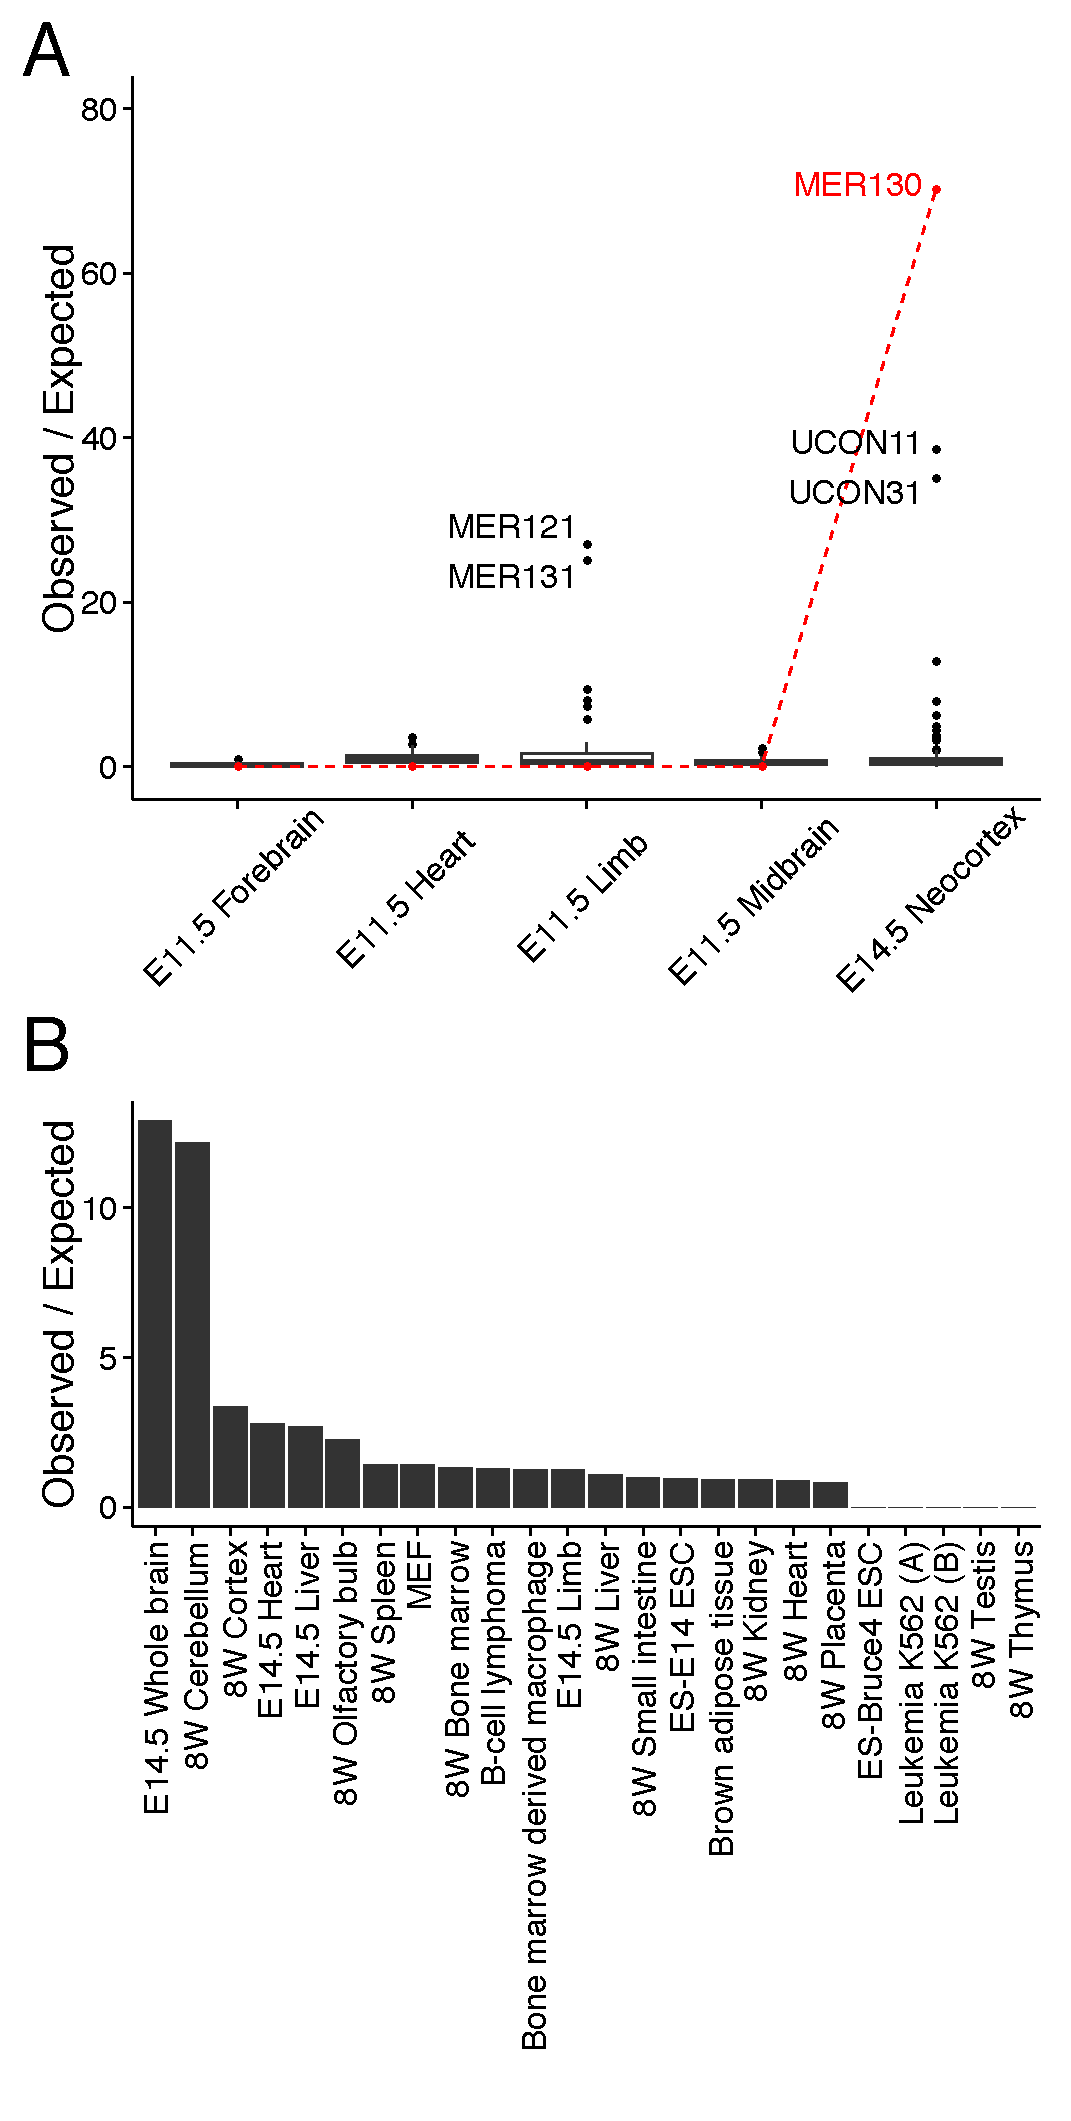
\epsfig{file=figures/mer130Figure1.pdf,width=0.5\linewidth,clip=,trim=0 0 0 0} \\
\end{tabular}
\caption[MER130 is strongly enriched among neocortical enhancers]{
{\bf MER130 is strongly enriched among neocortical enhancers.}
{\bf (A)} Fold enrichments compared to uniform shuffles for over
1,000 interspersed repeat families among p300 ChIP-seq datasets from
developing tissues. MER130 enrichments in red.
{\bf (B)} Fold enrichment of
observed MER130 instance overlaps compared to expected overlaps from
uniform shuffles of 24 ENCODE H3K27ac sets, including different primary
tissues at different developmental timepoints and model cell lines. No
enrichment comes close to the E14.5 neocortex enrichment in panel {\bf (A)}.
}
\label{fig:mer130Fig1}
\end{figure}

\subsection{MER130 is highly enriched among neocortex
enhancers}\label{mer130-is-highly-enriched-among-neocortex-enhancers}

Intrigued by the Britten \& Davidson hypothesis and encouraged by the
high specificity of the p300 mark, we asked whether any of
\textasciitilde{}1,000 known TE families are disproportionately marked
by an \emph{in vivo} p300 bound set of active enhancers (see Methods in \ref{sec:mer130Methods}).
One repeat family in one specific context stood out (\figref{fig:mer130Fig1}A): MER130 in
the E14.5 DCW with a 73 fold enrichment over expected (Bonferroni
p-value \textless{} 0.006, \emph{n} = 1,000,000 simulations)~\citep{Wenger:2013jd}.

Interestingly, MER130 was not enriched in any of a number of other p300
bound sequences from ChIP-seq experiments in other tissues, including
the forebrain at an earlier time-point (\figref{fig:mer130Fig1}A). The histone
modification H3K27ac, deposited by p300 at active
enhancers~\citep{Creyghton:2010hu}, is an easier-to-assay and thus more
comprehensively surveyed mark. We next searched for MER130 activity in
multiple additional tissues by performing the same enrichment test for
H3K27ac ChIP-seq sets from all 24 available tissues and cell lines from
the mouse Encyclopedia of DNA Elements (ENCODE)~\citep{ENCODEProjectConsortium:2012gc}. We
saw only weaker enrichments in other brain tissues: 12.9 fold enrichment
for E14.5 whole brain, 12.2 fold for 8-week cerebellum, and less than
4-fold enrichment in non-brain tissues (\figref{fig:mer130Fig1}B). Together, these data
show a strong enrichment for MER130 in E14.5 DCW, with more modest
enrichment in general brain tissue, compared to over 20 other tissue --
time point combinations.

\subsection{MER130 instances preserve a core regulatory
logic}\label{mer130-instances-preserve-a-core-regulatory-logic}
\begin{figure}[htbp]
\centering
\begin{tabular}{l}
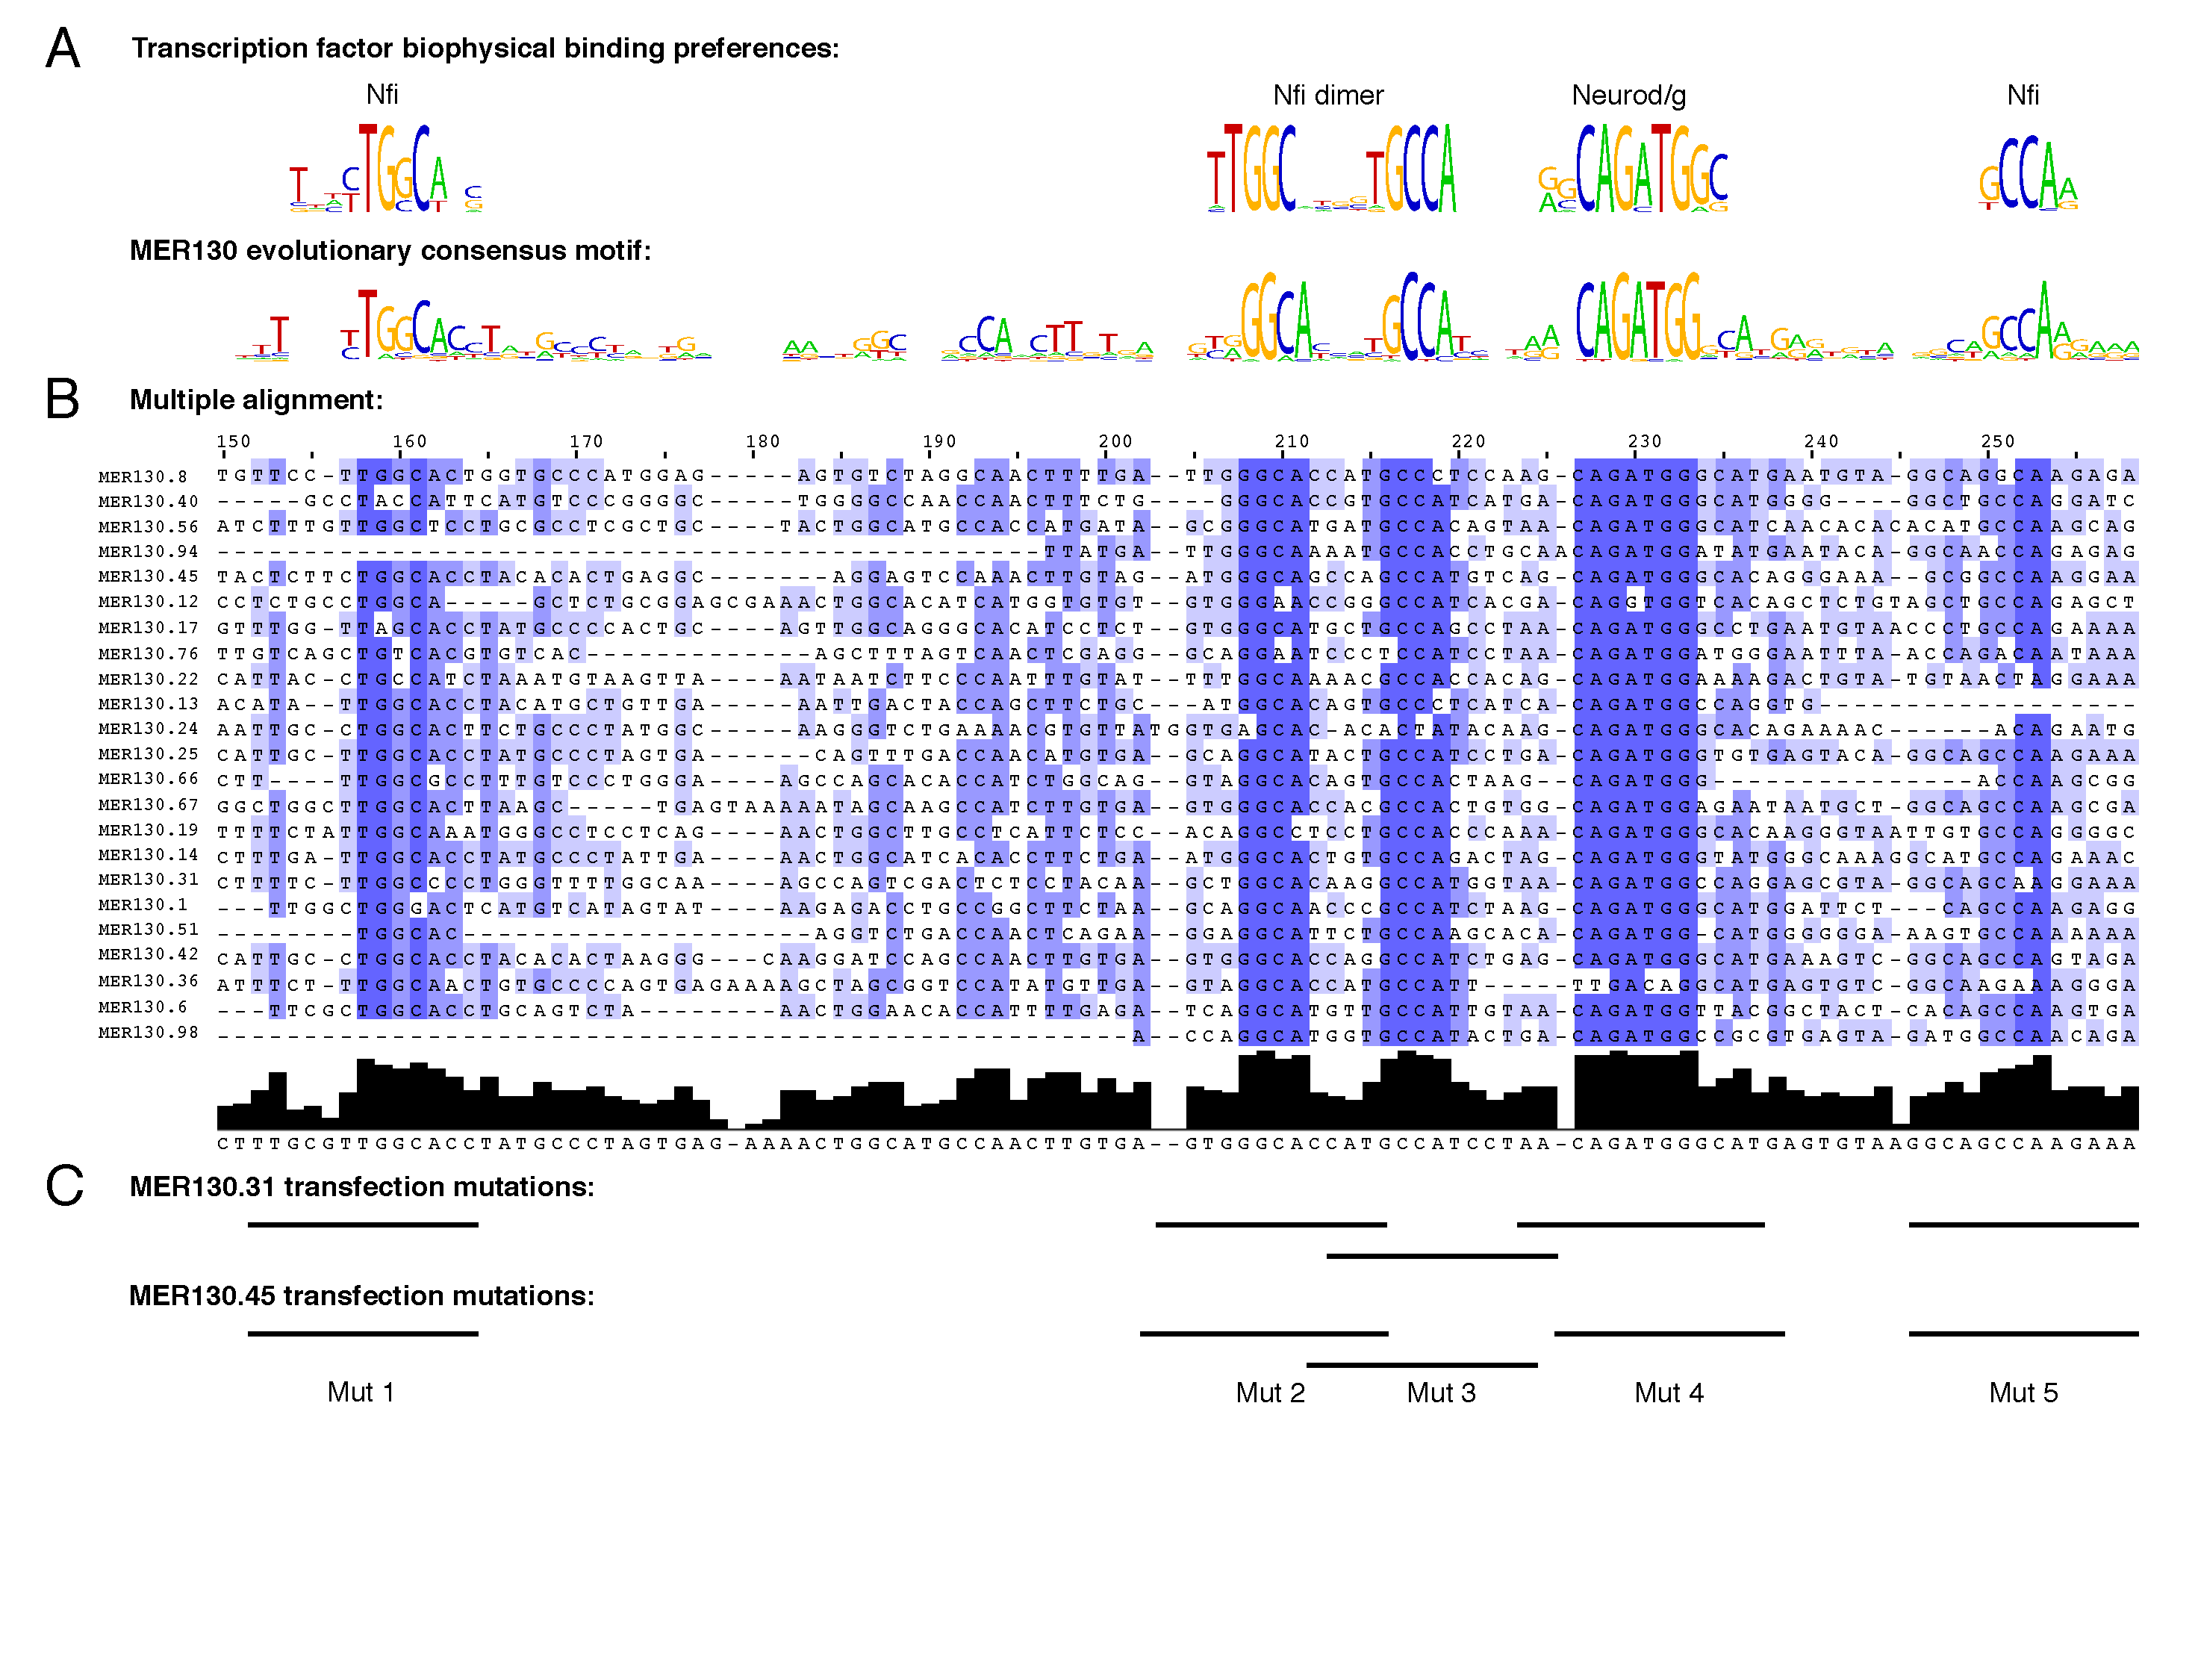
\epsfig{file=figures/mer130Figure2.pdf,width=0.99\linewidth,clip=,trim=0 0 0 0} \\
\end{tabular}
\caption[MER130 contains a preserved core of transcriptional regulatory logic]{
{\bf MER130 contains a preserved core of transcriptional regulatory logic.}
{\bf (A)} Biophysical transcription factor binding
preferences (top) and matching consensus motif (bottom) derived from
multiple alignment of MER130 instances marked by p300.
{\bf (B)} Multiple alignment of 23 MER130 instances strongly enriched for p300 signal.
{\bf (C)} Bases mutated in transfections (see \figref{fig:mer130Fig4}).
}
\label{fig:mer130Fig2}
\end{figure}

We next comprehensively annotated the MER130 family using nhmmer, a
probabilistic alignment tool~\citep{Wheeler:2013gj} (107 instances;
\tabref{tab:mer130TabS1}; see Methods in \ref{sec:mer130Methods}). Essentially all of the MER130
instances are distal (\textgreater{} 2.5 kb from the transcription start
site), and, as opposed to some other repeat
families~\citep{Bejerano:2006ep}, none overlap protein coding exons. We
identified 23 well-conserved MER130 instances that were strongly
enriched for the p300 ChIP-seq signal but not enriched for the input
control signal (see Methods in \ref{sec:mer130Methods}). Fourteen MER130 instances also overlap
E14.5 whole brain H3K27ac ChIP-seq peaks: 8 strongly marked by p300 in
our set and 6 marked with intermediate levels of p300. No instance
marked by low levels of p300 in our set was marked by H3K27Ac in E14.5
whole brain.

To achieve their specificity, enhancers contain distinct combinations of
transcription factor binding sites~\citep{Spitz:2012fj}. When we
constructed a multiple alignment from the 23 MER130 instances strongly
enriched for p300 signal, it revealed a well-conserved
\textasciitilde{}100 bp core (\figref{fig:mer130Fig2}B) containing 5 putative
transcription factor binding sites resembling motifs from our
library~\citep{Wenger:2013ds, Guturu:2013do}: a Neurod/Neurog motif, an Nfi
dimer~\citep{PortalesCasamar:2010db}, and two additional Nfi sites (\figref{fig:mer130Fig2}A),
representing families of factors important for brain development (see
Discussion in \ref{sec:mer130Discussion}).

\subsection{p300 marked MER130 instances function as
enhancers}\label{p300-marked-mer130-instances-function-as-enhancers}

\begin{figure}[htbp]
\centering
\begin{tabular}{l}
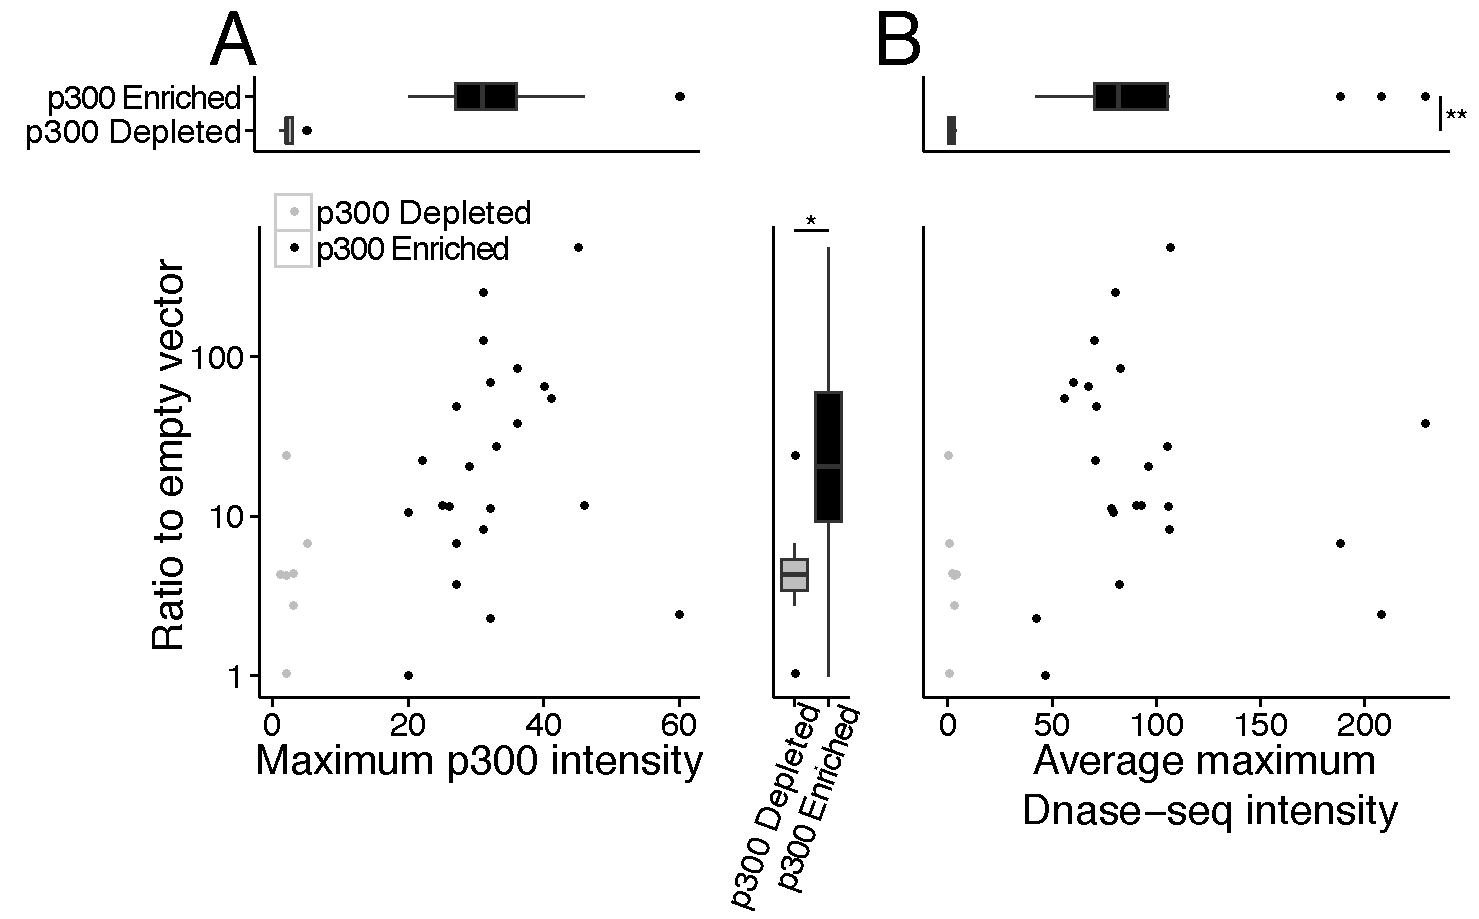
\epsfig{file=figures/mer130Figure3.pdf,width=0.99\linewidth,clip=,trim=0 0 0 0} \\
\end{tabular}
\caption[MER130 members function as enhancers but may not occupy open chromatin]{
{\bf MER130 members function as enhancers but may not occupy open chromatin.}
{\bf (A)} Maximum neocortex p300 ChIP-seq intensity
(x-axis) plotted against average fold activity relative to the empty
vector when transfected into dissociated cortical neurons (y-axis) for
each MER130 instance tested.
{\bf (B)} Average DNase-seq intensity across two
mouse E14.5 whole brain replicates (x-axis) plotted against same y-axis
as {\bf (A)} for the same set of MER130 instances. In both panels, MER130
elements enriched for the p300 signal in black (\emph{n =} 23) and
depleted for the p300 signal in gray (\emph{n =} 7). t-test. *p-value
\textless{} 0.05; **p-value \textless{} 0.01.
}
\label{fig:mer130Fig3}
\end{figure}

Next, we used our primary cortical neuron transfection system to test
whether the MER130 instances marked by p300 functioned as enhancers and
whether the binding sites preserved in the multiple alignment were
necessary for their activity (see Methods in \ref{sec:mer130Methods}). We cloned each of these 23
elements upstream of a minimal promoter and luciferase reporter, and
transfected these constructs into dissociated neurons isolated from
E14.5 mouse cortices (see Methods in \ref{sec:mer130Methods}). 22/23 (95.7\%) of the MER130
candidates hypothesized to function as neocortex enhancers produced
greater than 2-fold expression relative to the empty vector (\figref{fig:mer130Fig3}A, \figref{fig:mer130FigS1}).

Our result confirms that the MER130 instances marked by p300 function as
enhancers. While virtually all MER130 instances preserve the 5 binding
site core (\figref{fig:mer130FigS2}), over half (56 instances, 52\%) of
MER130 instances are clearly devoid of a DCW p300 mark (the remainder
show weak overlap, below our peak calling threshold; see Methods in \ref{sec:mer130Methods}). We
cloned 7 instances most depleted for p300 signal and tested them in the
same transfection assay. 6/7 (85.7\%) of these MER130 instances drove
\textgreater{} 2-fold expression relative to the empty vector, though at
a significantly weaker level than the set marked by p300 (p300 enriched,
\emph{n} = 23, to p300 depleted, \emph{n =} 7, \emph{t}-test \emph{p}-value: 0.03;
fold: 8.5; \figref{fig:mer130Fig3}A, \figref{fig:mer130FigS1}).

To better understand the \emph{in vivo} state of these sequences, we
examined the chromatin state from mouse E14.5 whole brain DNase-seq
data. Remarkably, the MER130 instances that were not marked by p300, yet
functioned as enhancers in dissociated cortical neurons, were
significantly (p300 enriched, \emph{n} = 23, to p300 depleted, \emph{n}
= 7, \emph{t}-test \emph{p}-value: 3.9e-09; fold: 51.7) depleted for DNaseI cleavage
when compared with the p300-marked MER130 instances that functioned in
transfection assays (\figref{fig:mer130Fig3}B).

Of the 107 MER130 instances we annotate in the mouse genome, 103 (96\%)
are conserved to human. We explored the chromatin state of these
conserved instances in day 85 human fetal brain tissue from the Roadmap
Epigenomics Project~\citep{Bernstein:2010cw}. Day 87 is the human time-point
matched to cortical neurogenesis in E14.5 mice~\citep{Clancy:2007fs}.
Strikingly, MER130 instances not marked by p300 occupied closed
chromatin not only in mouse, but also in human brain (\figref{fig:mer130FigS3}).

\begin{figure}[htbp]
\centering
\begin{tabular}{l}
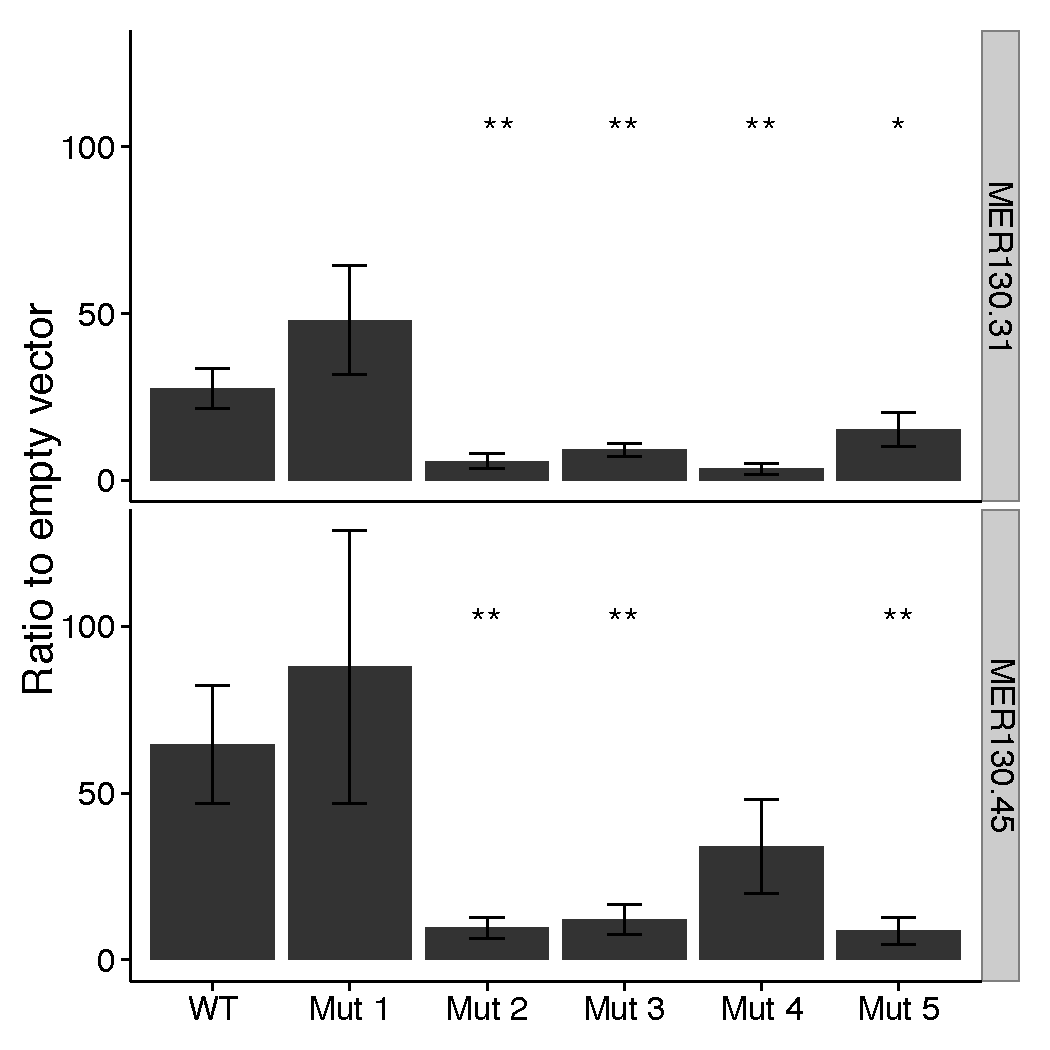
\epsfig{file=figures/mer130Figure4.pdf,width=0.6\linewidth,clip=,trim=0 0 0 0} \\
\end{tabular}
\caption[MER130 core mutations modulate enhancer activity
similarly across different instances]{
{\bf MER130 core mutations modulate enhancer activity
similarly across different instances.}
Two MER130 instances were mutated
each at 5 putative binding sites (nomenclature as in \figref{fig:mer130Fig2}C). Average
fold activity relative to the empty vector when mutated MER130 instances
were transfected into dissociated cortical neurons. Error bars represent
standard deviations. \emph{n} = 3 biological replicates x 3 technical
replicates for each condition. \emph{t}-test. *\emph{p}-value \textless{} 0.05;
**\emph{p}-value \textless{} 0.01. All 5 pairs trend in the same direction,
with 7/10 mutations significantly reducing expression.
}
\label{fig:mer130Fig4}
\end{figure}

We then tested the necessity of the preserved core for driving specific
expression levels in dissociated cortical neurons. Of the p300 enriched
MER130 instances robustly expressed in our transfection assay and
preserving the five binding sites, we chose two at random. We mutated
each of the 5 preserved binding sites in these two MER130 neocortex
enhancers (\figref{fig:mer130Fig2}C), and tested the resulting 10 constructs in our
primary cortical neuron transfection system. Mutating 7/10 (70\%)
predicted binding sites in the two enhancers resulted in a significant
reduction (wild-type to mutant fold change of 1.8-7.7) of reporter
activity (\figref{fig:mer130Fig4}).

\subsection{MER130 instances near critical neocortical development
genes}\label{mer130-instances-near-critical-neocortical-development-genes}

To identify functional coherence among the genes putatively regulated by
the MER130 neocortex enhancers, we analyzed them with
GREAT~\citep{McLean:2010iq}, a genomic region enrichment tool. We did not
observe any statistically significant enrichments for either the full
set of 107 MER130 elements or the set of 22 validated MER130 neocortex
enhancers. 6 of the 22 validated MER130 cortical enhancers, however, do
reside next to genes whose perturbations result in abnormal
telencephalon morphology: \emph{Robo1}, \emph{Id4}, \emph{Dgkb},
\emph{Ap3b1}, \emph{Prok2}, and \emph{Zfp423}. We also observed a second
MER130 instance marked by intermediate levels of p300 adjacent to two of
these six genes: \emph{Robo1} and \emph{Zfp423}. From the remaining
MER130 instances not enriched for p300 at E14.5, we observe MER130
instances next to 8 additional genes annotated with abnormal
telencephalon morphology: \emph{Cadm1}, \emph{Enah}, \emph{Epha4},
\emph{Foxg1}, \emph{Mycn}, \emph{Npas3}, \emph{Park2}, and
\emph{Pax3}~\citep{Eppig:2014ib}.

\subsection{MER130 originated in or before the tetrapod
ancestor}\label{mer130-originated-in-or-before-the-tetrapod-ancestor}

\begin{figure}[htbp]
\centering
\begin{tabular}{l}
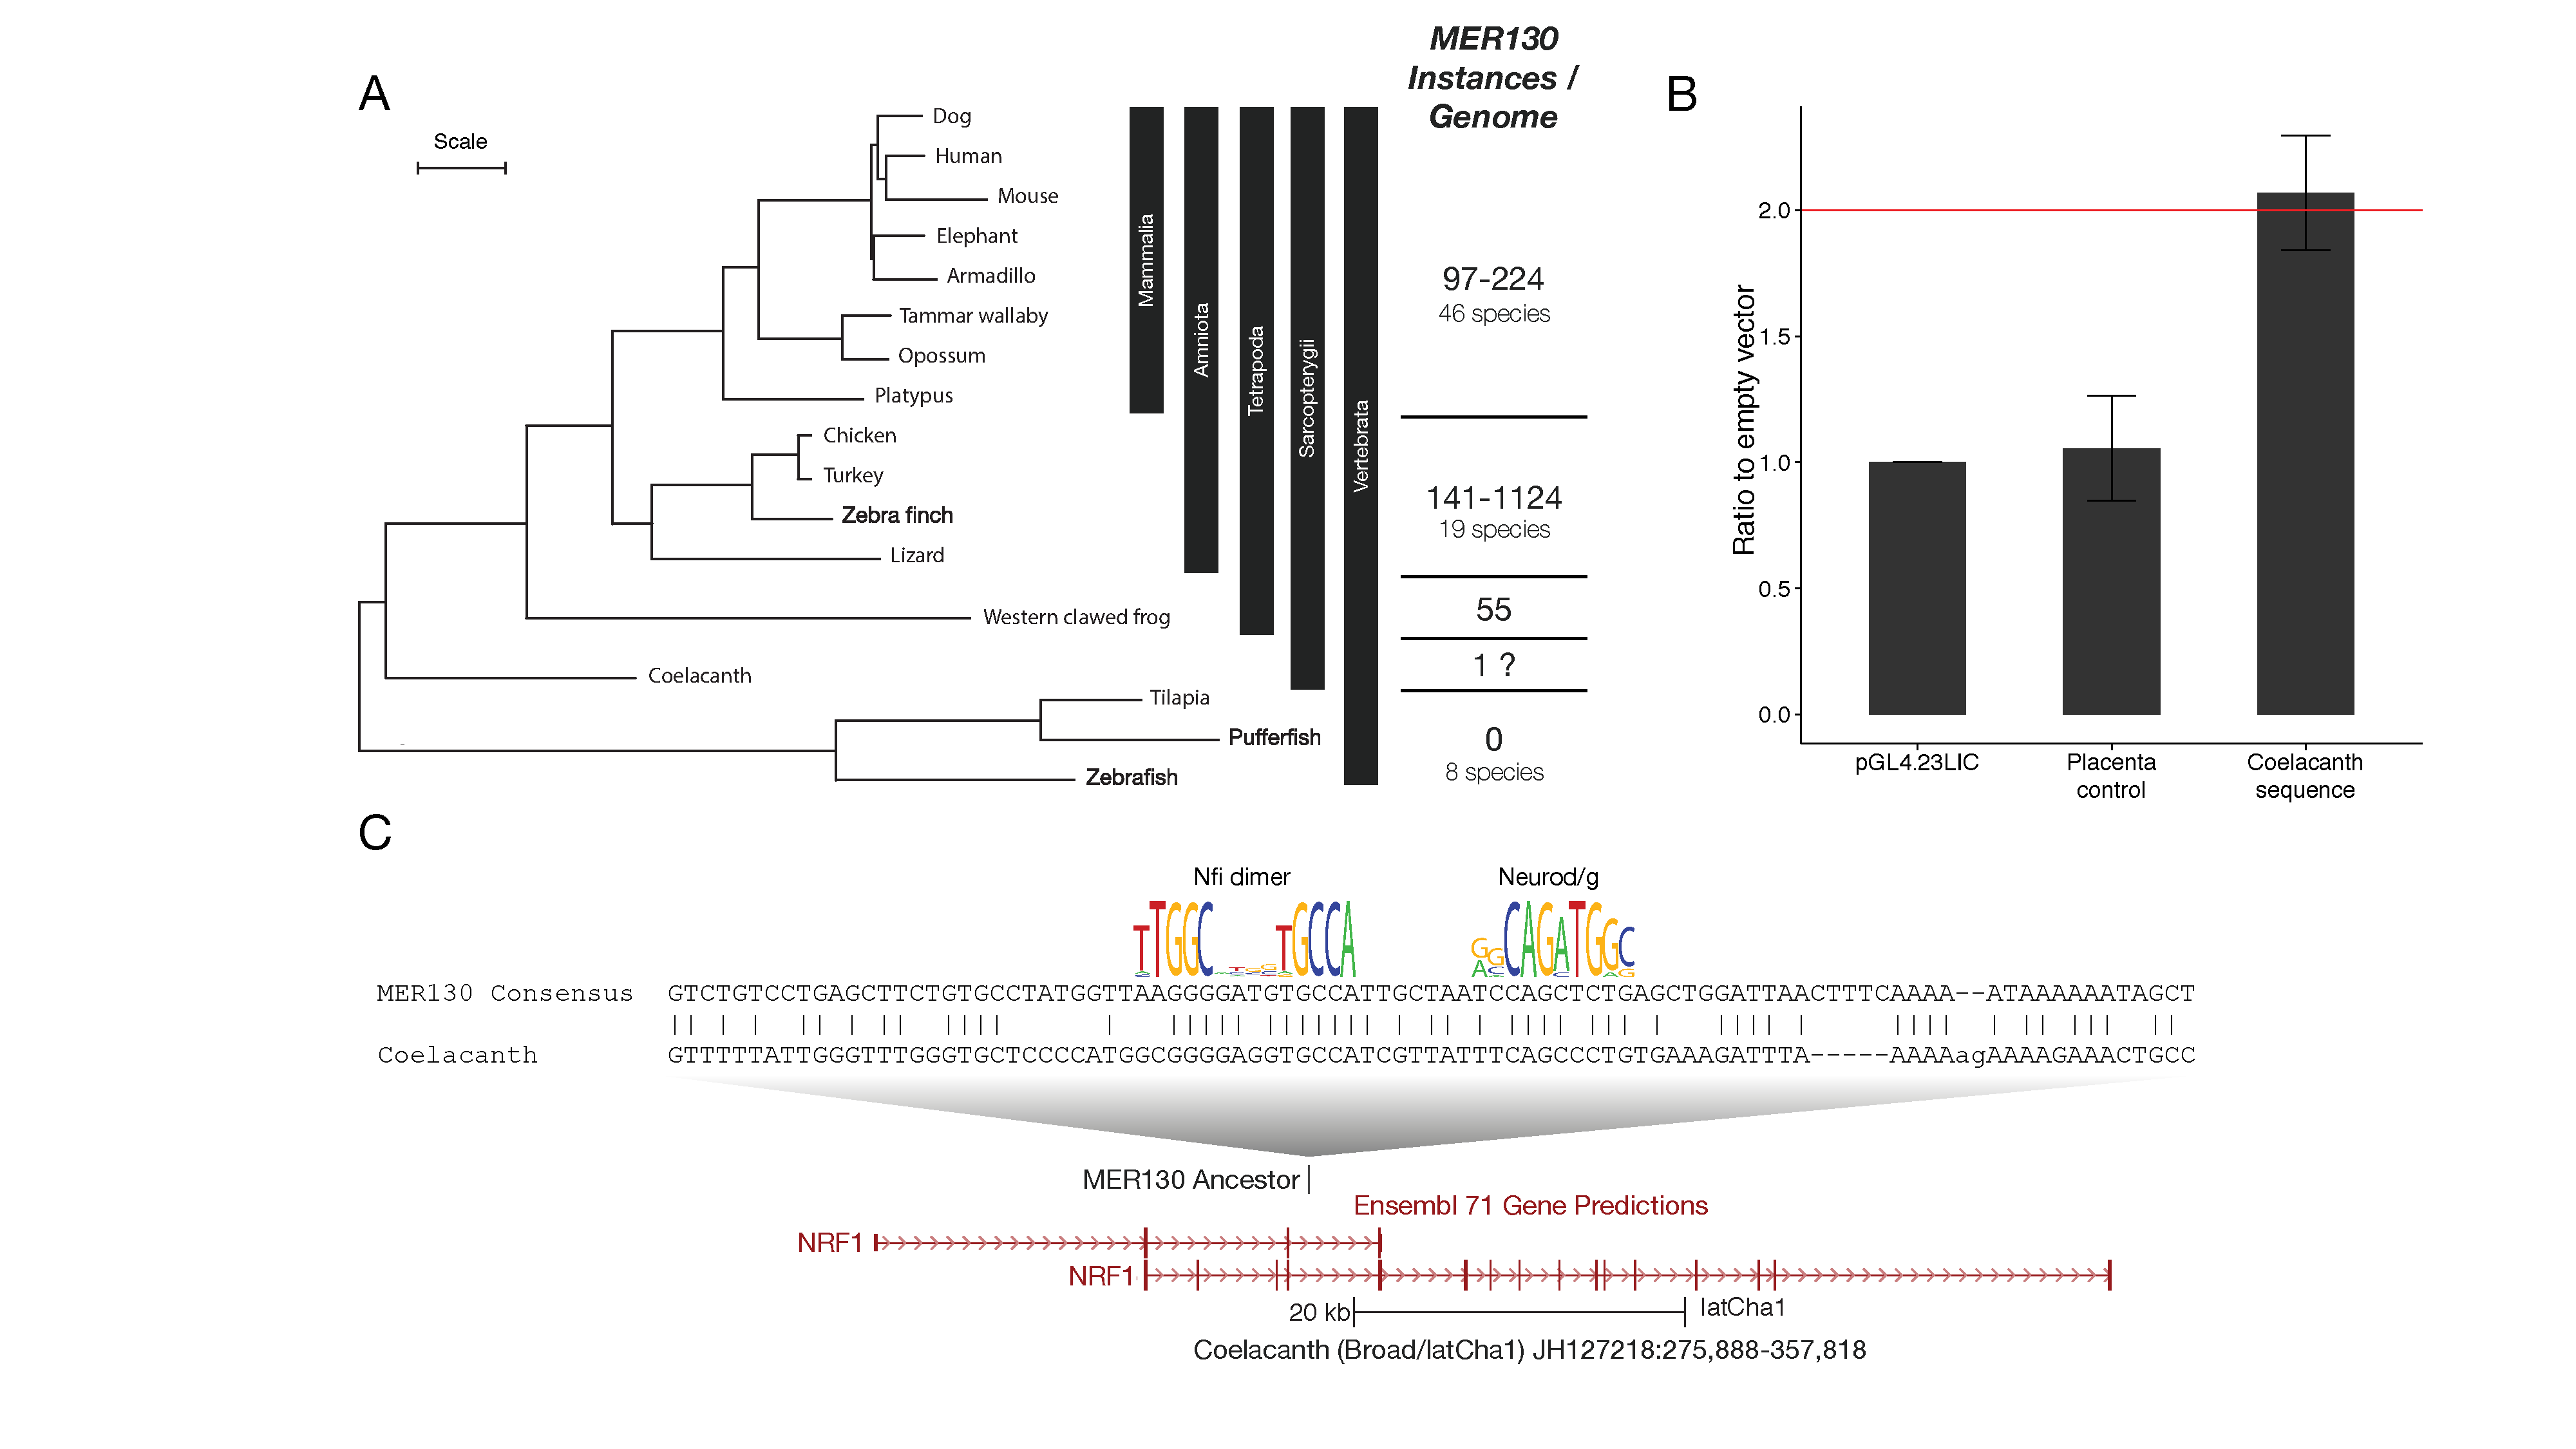
\epsfig{file=figures/mer130Figure5.pdf,width=0.99\linewidth,clip=,trim=0 0 0 0} \\
\end{tabular}
\caption[MER130 originated in the tetrapod or Sarcopterygii
ancestor]{
{\bf MER130 originated in the tetrapod or Sarcopterygii
ancestor.}
{\bf (A)} Phylogenetic tree (adapted from~\citep{Amemiya:2013hk}) with
representative species and the range of MER130 instances in species from
each clade. Scale: 0.1 substitutions per site.
{\bf (B)} Average fold activity
relative to the empty vector when the coelacanth sequence (panel {\bf (C)}) was
transfected into dissociated cortical neurons. Error bars represent
standard deviations.
{\bf (C)} Alignment between Dfam MER130 model and
Coelacanth genomic locus. Aligning bases preserve Nfi dimer and Neurod/g
motifs (\figref{fig:mer130Fig2}). The putative MER130 instance in coelacanth is located
in an intron of \emph{NRF1}, a gene that mediates neurite outgrowth.
}
\label{fig:mer130Fig5}
\end{figure}

The MER130 family is likely an interspersed repeat due to its consensus
length (\textasciitilde{}470 bp), composition, and distribution across
the genome~\citep{Bejerano:2006ep}. We queried all known repeat families and
databases of RNAs but found no homologous sequences that may help shed
light on the identity of MER130 (see Methods in \ref{sec:mer130Methods}). We also searched 75
vertebrate genome drafts and found no species with recent MER130
activity (\tabref{tab:mer130TabS2} and Methods in \ref{sec:mer130Methods}). While MER130 was
previously thought to originate in the amniote
ancestor~\citep{Jurka:2005bl}, we discovered that in fact it is conserved
in \emph{X. tropicalis}, suggesting this element originated no later
than the tetrapod ancestor (\figref{fig:mer130Fig5}A). We also identified a single
possible ancestral match in the Coelacanth genome (\figref{fig:mer130Fig5}C). This hit
occurs in the \emph{NRF1} ortholog, a gene that mediates neurite
outgrowth~\citep{Tong:2013bg}. Interestingly, despite the weak sequence
conservation, this coelacanth element drives greater than two-fold
activity when tested in dissociated cortical neurons (\figref{fig:mer130Fig5}B). No
MER130 matches were found in 7 species of bony fish or lamprey.

\subsection{Forebrain expression of genes near MER130
instances}\label{forebrain-expression-of-genes-near-mer130-instances}

Finally, we used the fact that MER130 is not present in fish to ask
whether the appearance of a MER130 instance next to a tetrapod gene
makes it more likely to be expressed in the forebrain than its ortholog
in fish. Using the GREAT default gene-region association rule, our 22
active MER130 instances can be associated with 37 immediately adjacent
genes. Seventeen of these genes, adjacent to 13 MER130 instances, are
annotated with ``TS21 - TS23 forebrain expression'' in
GXD~\citep{Eppig:2014ib}. Of the same 37 genes, we map 28 to orthologous
genes in zebrafish using the Ensembl ortholog mappings. Nineteen of
these are annotated for gene expression in any context in
ZFIN~\citep{Sprague:2006el}, and of them, only 3 genes are annotated for
forebrain expression. While anecdotal, these results suggest new gene
expression domains in the developing neocortex are associated with the
emergence of the MER130 family.

\section{Discussion}\label{sec:mer130Discussion}

The 73 fold enrichment of co-opted MER130 elements among E14.5 DCW
enhancers is striking. Similar magnitude enrichments have previously
only been reported in the context of embryonic stem
cells~\citep{Kunarso:2010kt,Jacques:2013jz}, with maximal folds in the twenties for
non-ES cell types or lines~\citep{Chuong:2013hj, Jacques:2013jz}. When we examined the
MER130 elements, we observed a clear core whose pattern of preservation
recapitulates the known biophysical binding preferences of two important
transcription factor families. The common activation code of Neurod/g
and Nfi binding sites are the likely reason for their recruitment as a
transcriptional network of neocortical enhancers. Together, these
features represent a striking example in support of the Britten \&
Davidson hypothesis.

Neurog and Nfi family members are promising candidates for
transcriptional regulators of MER130, given that \emph{Neurog2} mutant
mice, as well as mice null for \emph{Nfia}, \emph{Nfib}, and
\emph{Nfix}, all exhibit abnormal telencephalon morphology, the same
phenotype exhibited by mice null for multiple putative MER130 target
genes~\citep{Fode:2000ik, dasNeves:1999cn, SteelePerkins:2005kt, Campbell:2008ba}. The developing neocortex has been
microdissected at E14.5 to isolate the three layers present at this
timepoint, and gene expression in all three layers has been measured
using RNA-seq~\citep{Ayoub:2011jz}. Among \emph{Neurog} family members,
\emph{Neurog2} is the most highly expressed in all three layers at E14.5
and among \emph{Nfi} family members, \emph{Nfib} is the most highly
expressed in all three layers. Both genes are in the 1st percentile of
all expressed genes at this timepoint. The presence of four different
Nfi binding sites in the MER130 consensus further supports its
importance~\citep{Gotea:2010cc}.

While our experiments suggest that most MER130 instances are capable of
driving activity in the cortex, likely by virtue of their shared code,
the MER130 instances marked by p300 at E14.5 drive higher relative
activity when transfected in dissociated cortical neurons. In contrast
with the constructs we tested \emph{in vitro}, endogenous enhancer
activity also depends on the chromatin state~\citep{Arnold:2013di}. The
lack of DNaseI cleavage in both mouse and human brains suggests that the
MER130 instances not bound by p300 in our measurements are not only
weaker drivers in cortical neurons due to their sequence, but also
likely not accessible in their endogenous context.

MER130 is more ancient than previously thought. Our search of multiple
vertebrate genomes places its origin at least as early as the common
ancestor of tetrapods, possibly as early as our common ancestor with
coelacanth. The MER130 family exhibits an LF-SINE-like evolutionary
behavior where exapted copies shed revealing 5' and 3' marks, leaving
behind what is very likely only the body of the co-opted
transposon~\citep{Bejerano:2006ep}. We did not identify any instances
co-opted into coding exons, suggesting MER130 may not have ended in a
poly-A tail~\citep{Bejerano:2006ep}. The sequencing of additional tetrapod
genomes, especially genomically isolated ones, may yet reveal a species
with a recently jumping copy, allowing for the classification of this
repeat family~\citep{Lowe:2010ka}.

\section{Methods}
\label{sec:mer130Methods}

\subsection{All repeats -- p300 sets
correlation}\label{all-repeats-p300-sets-correlation}

We downloaded the RepeatMasker track from the pre-annotated mm9 genome
(RepeatMasker open-3.2.8 Repeat Library)~\citep{Smit:OL9JT8qH} and
removed low-complexity, satellite, and simple repeat classes, while
retaining DNA, LINE, SINE, LTR, and RNA classes for a total of 1,118
repeat and RNA families. We next downloaded p300 ChIP-seq results for
E11.5 forebrain~\citep{Visel:2013it}, midbrain, heart, and
limb~\citep{Blow:2010bu} and removed proximal peaks (\textless{}2.5 kb
away from any TSS in UCSC knownGene track). We shuffled each p300 set
across the genome 10,000 times (excluding the UCSC mm9 gap track). For
each p300 set shuffle, we counted the number of p300 set instances
overlapped by each repeat family. We also computed the number of actual
p300 set instances overlapped by each repeat family. Fold enrichment was
computed as observed divided by mean for each repeat family - p300 set
combination. To better estimate the \emph{p}-value for the enrichment of the
MER130 family and determine statistical significance, we performed an
additional 1,000,000 shuffles of our neocortex p300 set against this
repeat family alone.

\subsection{Tissue specificity}\label{tissue-specificity}

We downloaded all 24 available H3K27ac tissue and cell-line data from
ENCODE and removed all peaks overlapping an exon (UCSC mm9.knownGene)
and proximal peaks (\textless{}2.5 kb away from any TSS). Observed and
expected overlaps were computed as above.

\subsection{MER130 instances identification and intersection with
p300}\label{mer130-instances-identification-and-intersection-with-p300}

We used nhmmer (from hmmer3.1-snap20121011 using -\/-cut-ga threshold)~\citep{Wheeler:2013gj} to identify 107 instances of the MER130 repeat
family in the mouse genome (NCBI37/mm9), using Dfam's MER130 DF0000726.2
profile HMM model~\citep{Wheeler:2012im}. Each MER130 instance was
semi-automatically classified as high, medium, or low confidence based
on computing maximum p300 signal intensity over each peak, followed by
manual inspection. Read pileups were constructed using MACS1.4, and the
maximum peak height was extracted using UCSC bigWigAverageOverBed.
Maximum p300 read pileup from the p300 ChIP-seq was used as the primary
selection attribute, and instances classified as high confidence had a
punctuated peak over the MER130 family member, as well as low input
control signal. This resulted in 23 well-conserved MER130 instances with
maximum p300 read pileup height \textgreater{}= 20 (high), 28 instances
marked by intermediate levels of p300 (7 \textless{}= p300 \textless{}=
24 ; medium), and 56 instances marked by background levels of p300 (0
\textless{}= p300 \textless{}= 6; low).

\subsection{Multiple alignment}\label{multiple-alignment}

Sequences aligning to the DFAM DF0000726.2 profile HMM model
(corresponding to the 23 MER130 instances strongly enriched for p300
signal) were extracted from the mouse genome (NCBI37/mm9). A multiple
alignment of these sequences was then constructed using MUSCLE (v3.8.31)~\citep{Edgar:2004bo}.

\subsection{Ethics}\label{ethics}

All animal work was carried out in compliance with the Stanford
University Institutional Animal Care and Use Committee under approved
protocols \#18487 and \#21758. Timed pregnant female mice were adults
greater than six weeks of age and maintained on a Swiss Webster
background (Charles River). Embryos at the time of harvest were 14.5
days post coitum.

\subsection{Cloning and transfections}\label{cloning-and-transfections}

Cloning and transfections were performed as in~\citep{Wenger:2013ds}.
Briefly, inserts were amplified from mouse genomic DNA (Clonetech
Laboratories Inc.) using Phusion High Fidelity DNA Polymerase (NEB
Inc.). For transfections using the coelacanth match to the MER130
consensus, a 196 bp insert containing the MER130 core match was
amplified from coelacanth (\emph{Latimeria menadoensis)} genomic DNA. A
Ligation Independent Cloning (LIC) site was ligated to the firefly
luciferase vector, PGL4.23 (Promega Corp.), at the 5' KpnI and 3'
HindIII sites, and all inserts were cloned into the PGL4.23 LIC vector
using an LIC method~\citep{Du:2011cf}. All positive clones were
identified by colony PCR and sequenced. E14.5 embryos were harvested
from Swiss Webster mice (Charles River). The dorsal telencephalon was
removed and stored briefly on ice in an HBSS dissection solution. Cells
were dissociated using 0.25\% trypsin and 10ug/ul DNase. Nucleofections
were performed using the experimental luciferase construct and a pRL-CMV
Renilla control (Promega) and a P3 Primary Cell 96-well Nucleofector Kit
(Lonza). Nucleofected cells were plated onto poly-D-lysine coated
96-well plates (NUNC) containing PNBM (Lonza). Luciferase assays were
performed 48 hours after nucleofection using the Dual-Luciferase®
Reporter 1000 Assay System (Promega) according to the manufacturer's
protocol and read using a Promega Glomax luminometer. An enhancer
sequence that drove activity in placental cells, but not in cortical
neurons in luciferase reporter assays~\citep{Tuteja:2014cw}, was used as a
negative control. Primers are listed in \tabref{tab:mer130TabS3}.

\subsection{Site directed mutagenesis}\label{site-directed-mutagenesis}

Site-directed mutagenesis was performed as in~\citep{Camp:2012dh}.
Briefly, the PGL4.23 LIC vector containing the normal insert served as
the template for short cycle PCR using specially designed primers and
Phusion High Fidelity DNA Polymerase (NEB Inc.). DpnI was used to digest
the template. All clones were identified by colony PCR and sequenced.
Primers are listed in \tabref{tab:mer130TabS3}.

\subsection{Chromatin state}\label{chromatin-state}

Day 85 human fetal brain tissue DNase-seq intensities were downloaded
from the Roadmap Epigenomics Project~\citep{Bernstein:2010cw}. Mouse
sequences were lifted to human using the UCSC liftOver tool
(-minMatch=0.2), and the maximum peak height was measured using UCSC
bigWigAverageOverBed.

\subsection{Genomic region enrichment
analysis}\label{genomic-region-enrichment-analysis}

Enrichment analysis was performed using GREAT
(\url{http://great.stanford.edu/}) version 2.0.2~\citep{McLean:2010iq}
with default parameters.

\subsection{MER130 origins and activity}

Sequences were queried using nhmmer~\citep{Wheeler:2013gj} (from
hmmer3.1-snap20121011 using -\/-cut-ga threshold) with the
Dfam~\citep{Wheeler:2012im} MER130 DF0000726.2 profile HMM model.

We first searched the RepBase catalog of repeats~\citep{Jurka:2005bl}, to
identify homologous repeat families, as well as the eukaryotic tRNA
database~\citep{Chan:2009dz} and Rfam~\citep{Burge:2013bs} to probe for
RNAs from which a SINE element may have been
derived~\citep{Bejerano:2006ep}. We then downloaded vertebrate genome
sequences from UCSC
(\url{http://hgdownload.cse.ucsc.edu/downloads.html})
and vertebrate scaffolds from Genbank Release 196
(\url{ftp://ftp.ncbi.nlm.nih.gov/genbank/genomes/Eukaryotes/vertebrates\_other/}).

A total of 75 available vertebrate genome drafts were searched. We
observed repeat densities of 0.0-0.5 copies per megabase (Mb) (\figref{fig:mer130Fig5}A,
\tabref{tab:mer130TabS2}). The green sea turtle, with the highest repeat
density of a modest 0.5 copies per Mb, had 1,124 MER130 copies present
in its genome (\figref{fig:mer130Fig5}A, \tabref{tab:mer130TabS2}). However, these instances
were quite diverged from each other, suggesting that MER130 has long
been inactive in this lineage as well~\citep{Bejerano:2006ep, Kazazian:2004bf}.
